\documentclass{beamer}

\usepackage[utf8]{inputenc}
\usepackage{default}
\usepackage{multicol}
\usetheme{Warsaw}
\usecolortheme{seahorse}
\useoutertheme{shadow}
\useinnertheme{rectangles}

\title[Fibonacci Heap]{Fibonacci Heap}
\author[ALMA\and *Alexis\and Luis \and Margarita \and Ademir*]{{Bernal Chauayo, Luis Antonio}\\{Lacuaña Apaza, Margarita}\\{Mendoza Villarroel, Alexis}\\{Villena Zevallos, Ademir}}
\institute{{Ciencia de la Computación}
\\{Universidad Nacional de San Agustin}}
\date{2 de Octubre del 2016}

\begin{document}

\begin{frame}[plain]
    \titlepage
 \end{frame}
  
 \begin{frame}
  \frametitle{Índice}
  \begin{multicols}{2}
  \tableofcontents
  \end{multicols} 
\end{frame}

\section{Historia}
\begin{frame}
    \frametitle{Historia}
 \begin{itemize}
    \item Los Fibonacci heap  fueron desarrollados en 1984 por Michael L. Fredman y Robert E. Tarjan.
    \item Publicados por primera vez en una revista científica en 1987.
    \item El nombre de montículos de Fibonacci viene de la sucesión de Fibonacci, que se usa en pruebas comparativas de tiempo (Benchmarking).
\end{itemize}
\end{frame}

\section{Insertar}
\begin{frame}
  \frametitle{Insertar}
  \begin{columns}[t]
    \column{0.5\textwidth}
    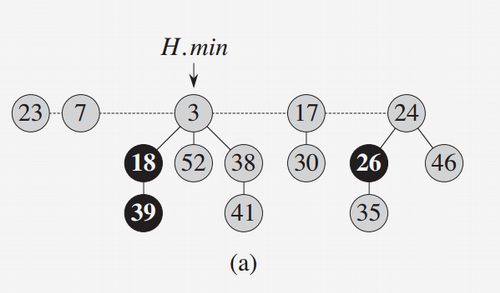
\includegraphics[width =1 \textwidth]{imagenes/insertar1.png}
      
    \column{0.5\textwidth}
    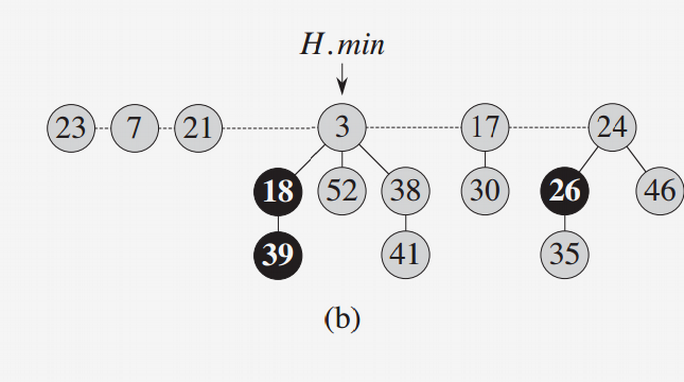
\includegraphics[width =1 \textwidth]{imagenes/insertar2.png}

   \end{columns}
  
\end{frame}


\section{GetMin}
\begin{frame}
  \frametitle{GetMin}
  \begin{itemize}
    \item El mínimo nodo de un Fibonacci Heap está dado por el puntero H.min así que podemos encontrarlo en O(1) . 
  \end{itemize}
  
   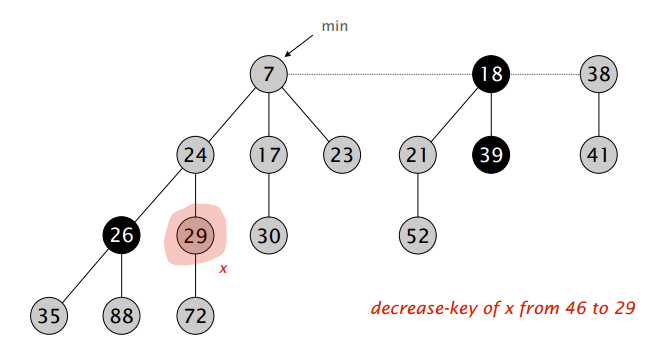
\includegraphics[width =1 \textwidth]{img/decrease/01.png}

\end{frame}

\section{DecreaseKey}
\begin{frame}
  \frametitle{DecreaseKey}
  \framesubtitle{Caso 1: Orden del hep correcto}
  \begin{itemize}
    \item Decrementar el dato de X
    \item Actualizar puntero H.min (Si es necesario)

  \end{itemize}
  
   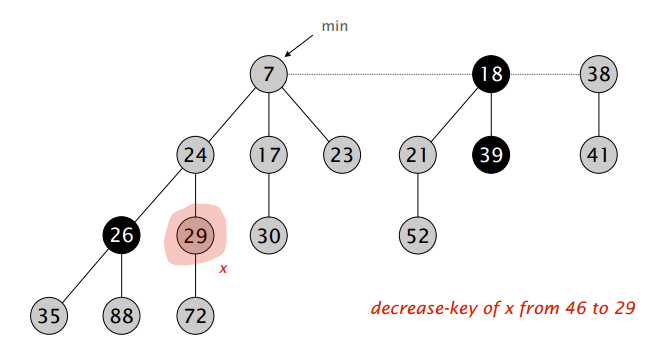
\includegraphics[width =1 \textwidth]{img/decrease/01.png}
\end{frame}



\begin{frame}
  \frametitle{DecreaseKey}
  \framesubtitle{Caso 2: Orden del hep incorrecto}
  \begin{itemize}
    \item Decrementar el dato de X
  \end{itemize}
     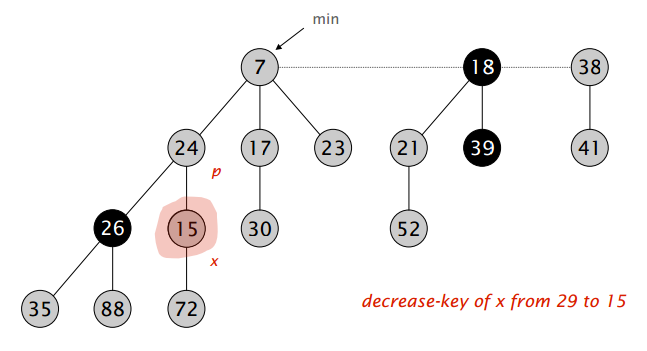
\includegraphics[width =1 \textwidth]{img/decrease/02.png}
\end{frame}


\begin{frame}
  \frametitle{DecreaseKey}
  \framesubtitle{Caso 2: Orden del hep incorrecto}
  \begin{itemize}
    \item Cortar árbol en x, agregar a la lista de raíces y desmarcar.
  \end{itemize}
     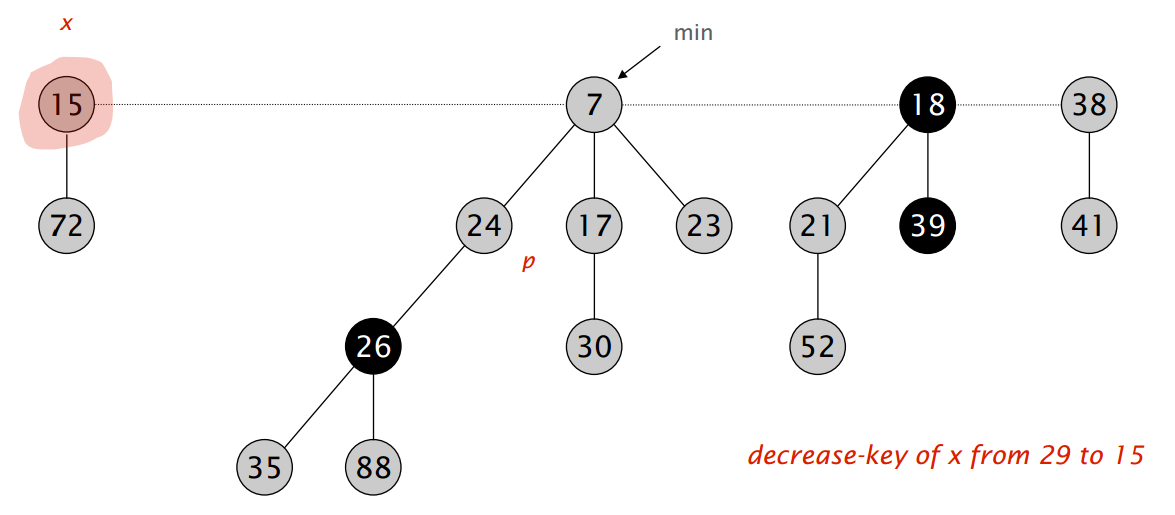
\includegraphics[width =1 \textwidth]{img/decrease/03.png}
\end{frame}


\begin{frame}
  \frametitle{DecreaseKey}
  \framesubtitle{Caso 2: Orden del hep incorrecto}
  \begin{itemize}
    \item Si el padre p de x esta desmarcado (No ha perdido un hijo aun), marcar este; En otro caso cortar p, unirlo a la lista de raíces y desmarcarlo. (Hacer esto recursivamente para todos los ancestros que perdieron un segundo hijo).
  \end{itemize}
     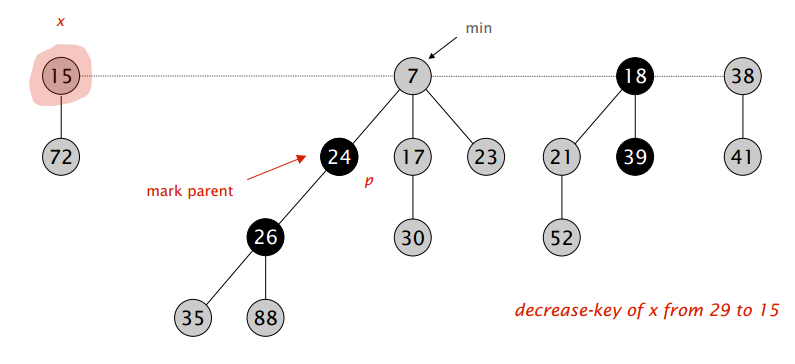
\includegraphics[width =1 \textwidth]{img/decrease/04.png}
\end{frame}


\begin{frame}
  \frametitle{DecreaseKey}
  \framesubtitle{Ejemplo}
   
     \begin{columns}[t]
    \column{0.5\textwidth}
    \centering
    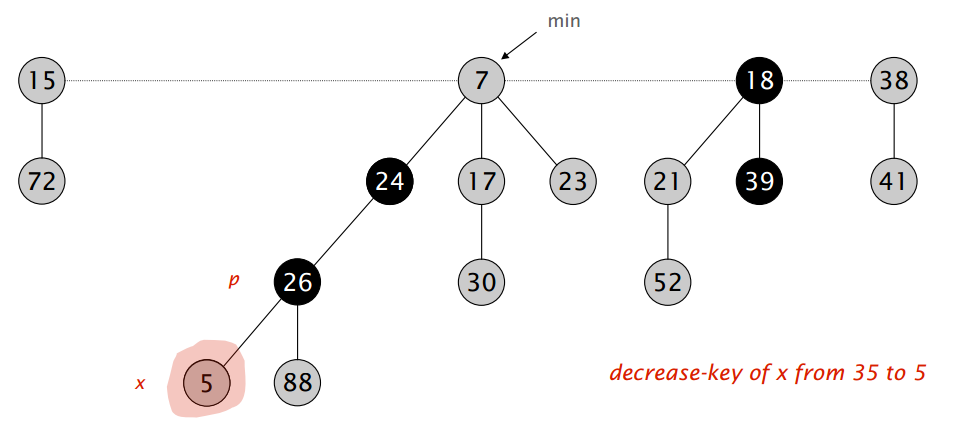
\includegraphics[width =1 \textwidth]{img/decrease/05.png} \\
    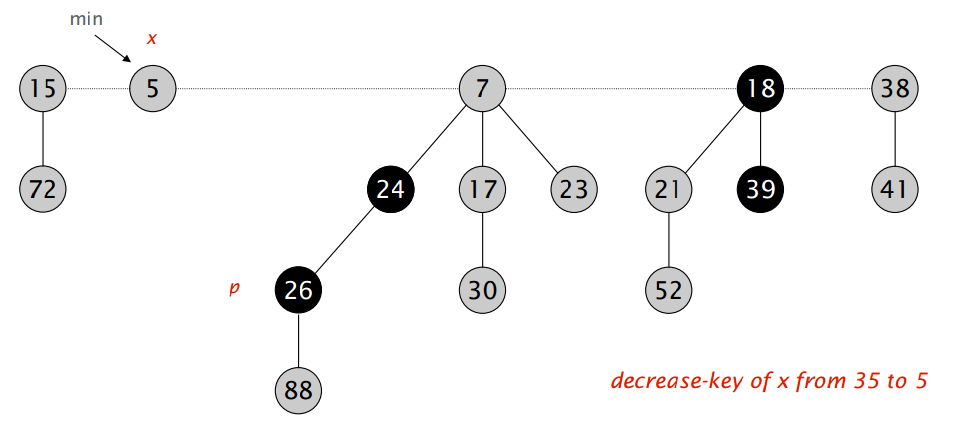
\includegraphics[width =1 \textwidth]{img/decrease/06.png}
      
    \column{0.5\textwidth}
    \centering
    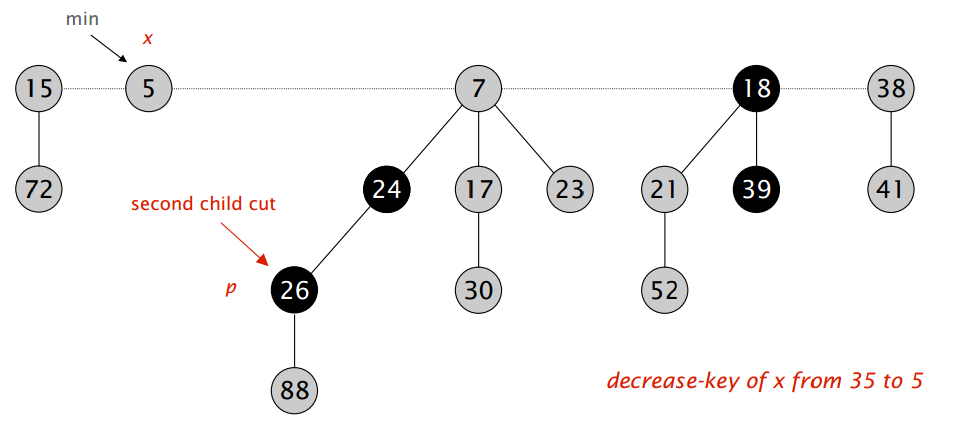
\includegraphics[width =1 \textwidth]{img/decrease/07.png} \\
    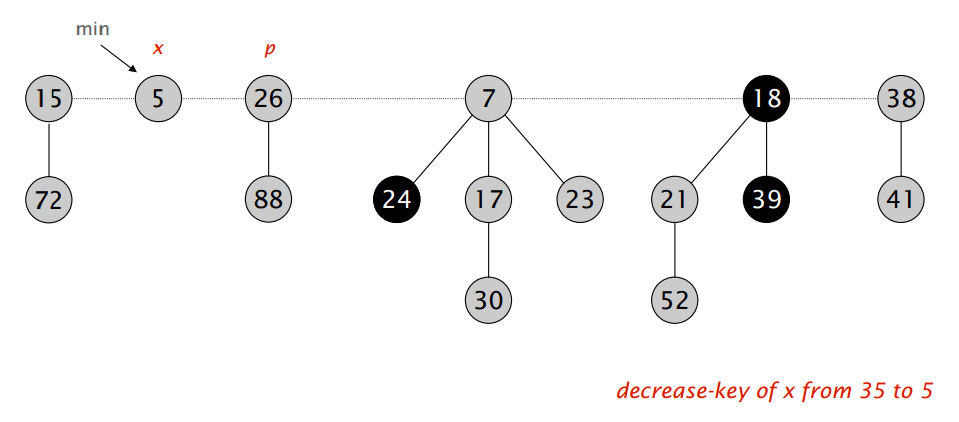
\includegraphics[width =1 \textwidth]{img/decrease/08.png}

   \end{columns}
   
\end{frame}


\begin{frame}
  \frametitle{DecreaseKey}
  \framesubtitle{Ejemplo}
   
     \begin{columns}[t]
    \column{0.5\textwidth}
    \centering
    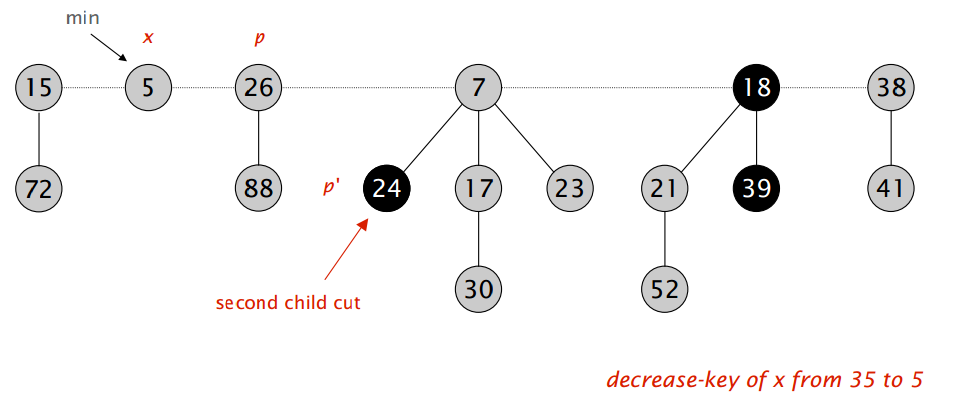
\includegraphics[width =1 \textwidth]{img/decrease/09.png} 
      
    \column{0.5\textwidth}
    \centering
    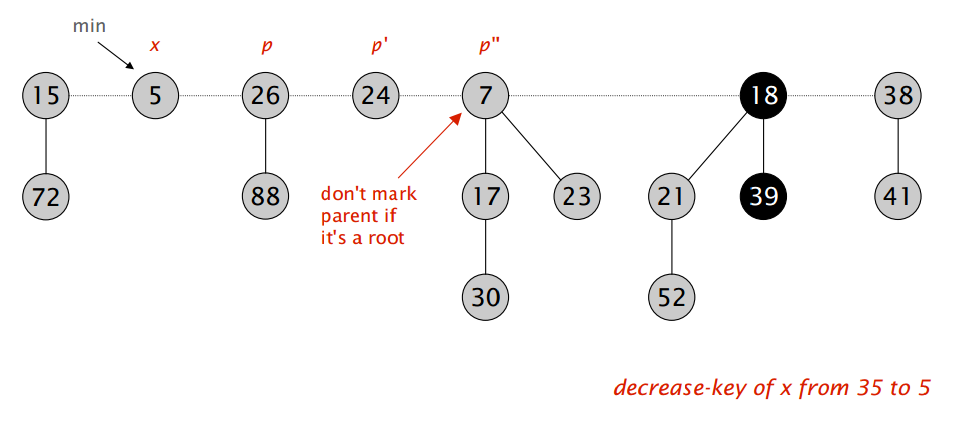
\includegraphics[width =1 \textwidth]{img/decrease/10.png} 

   \end{columns}
   
\end{frame}


\end{document}
